% Graphic for TeX using PGF
% Title: D:\Dropbox\Master Thesis\Smart Cafeteria Report\src\ch3\ClassDiagram\ClassDiagram.dia
% Creator: Dia v0.97.2
% CreationDate: Mon May 27 13:02:26 2013
% For: Richard
% \usepackage{tikz}
% The following commands are not supported in PSTricks at present
% We define them conditionally, so when they are implemented,
% this pgf file will use them.
\ifx\du\undefined
  \newlength{\du}
\fi
\setlength{\du}{15\unitlength}
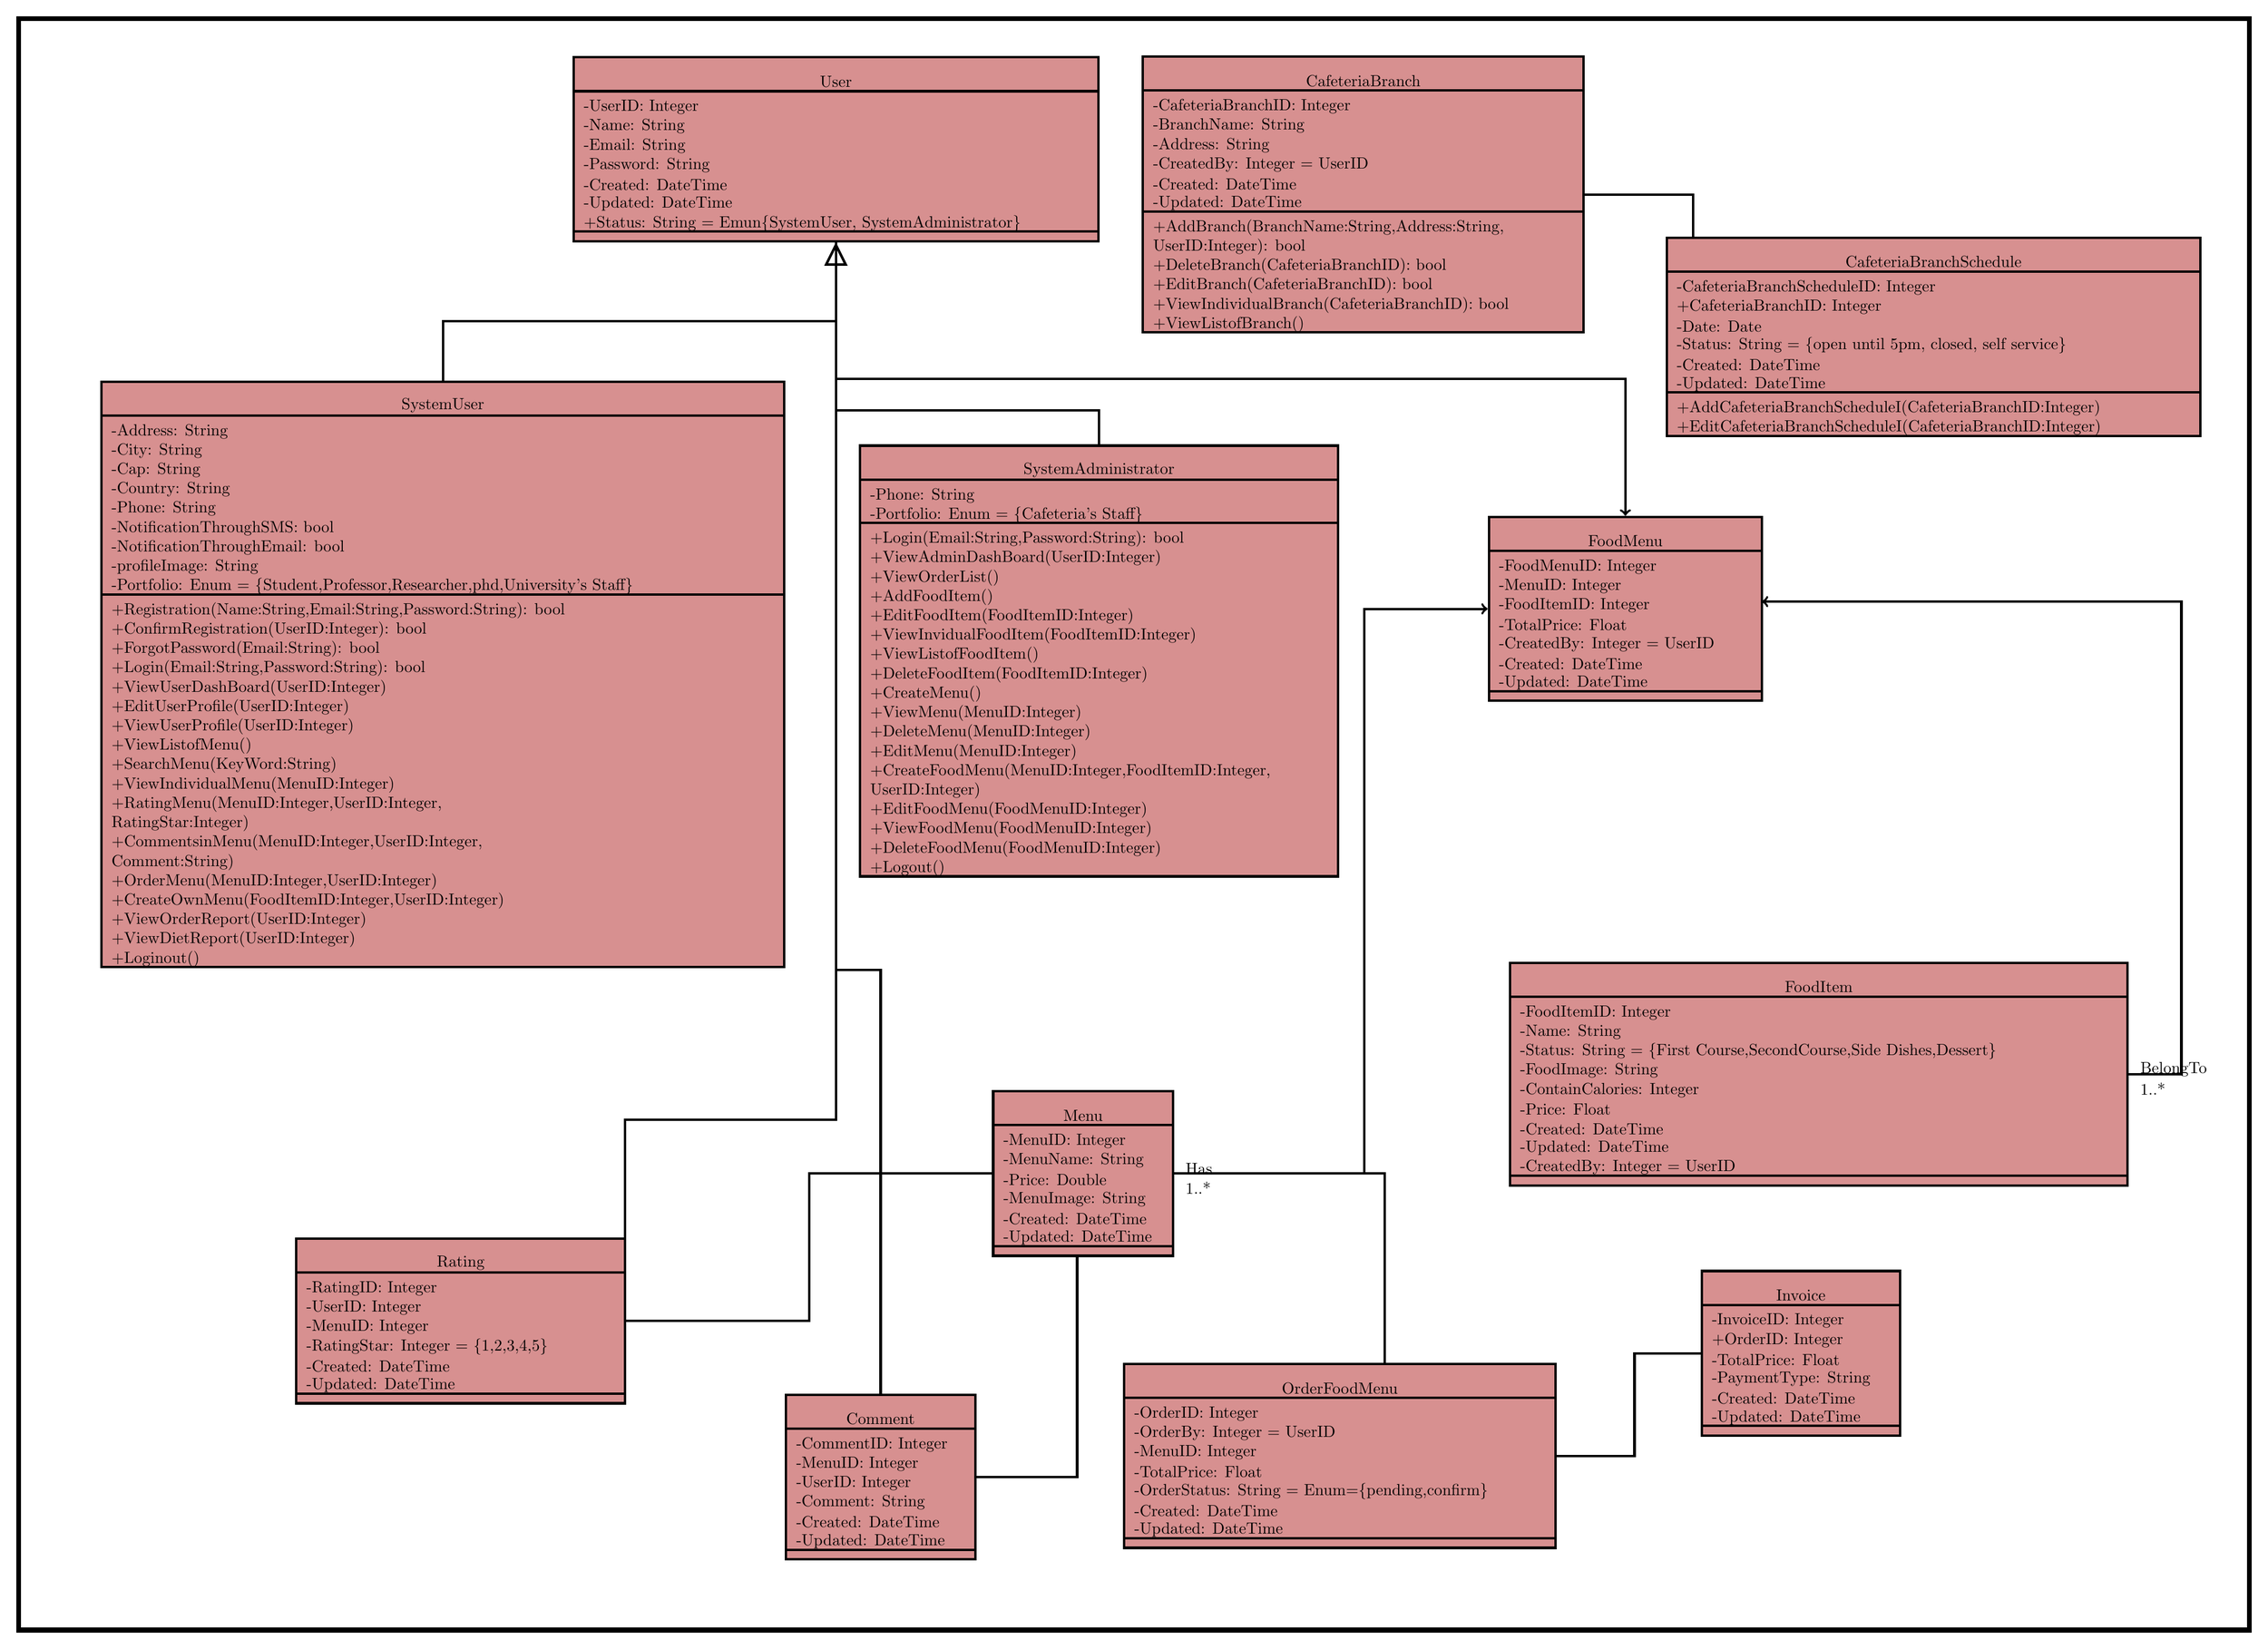
\begin{tikzpicture}
\pgftransformxscale{1.000000}
\pgftransformyscale{-1.000000}
\definecolor{dialinecolor}{rgb}{0.000000, 0.000000, 0.000000}
\pgfsetstrokecolor{dialinecolor}
\definecolor{dialinecolor}{rgb}{1.000000, 1.000000, 1.000000}
\pgfsetfillcolor{dialinecolor}
\pgfsetlinewidth{0.200000\du}
\pgfsetdash{}{0pt}
\pgfsetdash{}{0pt}
\pgfsetmiterjoin
\definecolor{dialinecolor}{rgb}{1.000000, 1.000000, 1.000000}
\pgfsetfillcolor{dialinecolor}
\fill (-30.557400\du,-92.525400\du)--(-30.557400\du,-25.925400\du)--(61.609968\du,-25.925400\du)--(61.609968\du,-92.525400\du)--cycle;
\definecolor{dialinecolor}{rgb}{0.000000, 0.000000, 0.000000}
\pgfsetstrokecolor{dialinecolor}
\draw (-30.557400\du,-92.525400\du)--(-30.557400\du,-25.925400\du)--(61.609968\du,-25.925400\du)--(61.609968\du,-92.525400\du)--cycle;
\pgfsetlinewidth{0.100000\du}
\pgfsetdash{}{0pt}
\definecolor{dialinecolor}{rgb}{0.843137, 0.564706, 0.564706}
\pgfsetfillcolor{dialinecolor}
\fill (-27.135700\du,-77.520500\du)--(-27.135700\du,-76.120500\du)--(1.084300\du,-76.120500\du)--(1.084300\du,-77.520500\du)--cycle;
\definecolor{dialinecolor}{rgb}{0.000000, 0.000000, 0.000000}
\pgfsetstrokecolor{dialinecolor}
\draw (-27.135700\du,-77.520500\du)--(-27.135700\du,-76.120500\du)--(1.084300\du,-76.120500\du)--(1.084300\du,-77.520500\du)--cycle;
% setfont left to latex
\definecolor{dialinecolor}{rgb}{0.000000, 0.000000, 0.000000}
\pgfsetstrokecolor{dialinecolor}
\node at (-13.025700\du,-76.520500\du){SystemUser};
\definecolor{dialinecolor}{rgb}{0.843137, 0.564706, 0.564706}
\pgfsetfillcolor{dialinecolor}
\fill (-27.135700\du,-76.120500\du)--(-27.135700\du,-68.720500\du)--(1.084300\du,-68.720500\du)--(1.084300\du,-76.120500\du)--cycle;
\definecolor{dialinecolor}{rgb}{0.000000, 0.000000, 0.000000}
\pgfsetstrokecolor{dialinecolor}
\draw (-27.135700\du,-76.120500\du)--(-27.135700\du,-68.720500\du)--(1.084300\du,-68.720500\du)--(1.084300\du,-76.120500\du)--cycle;
% setfont left to latex
\definecolor{dialinecolor}{rgb}{0.000000, 0.000000, 0.000000}
\pgfsetstrokecolor{dialinecolor}
\node[anchor=west] at (-26.985700\du,-75.460500\du){-Address: String};
% setfont left to latex
\definecolor{dialinecolor}{rgb}{0.000000, 0.000000, 0.000000}
\pgfsetstrokecolor{dialinecolor}
\node[anchor=west] at (-26.985700\du,-74.660500\du){-City: String};
% setfont left to latex
\definecolor{dialinecolor}{rgb}{0.000000, 0.000000, 0.000000}
\pgfsetstrokecolor{dialinecolor}
\node[anchor=west] at (-26.985700\du,-73.860500\du){-Cap: String};
% setfont left to latex
\definecolor{dialinecolor}{rgb}{0.000000, 0.000000, 0.000000}
\pgfsetstrokecolor{dialinecolor}
\node[anchor=west] at (-26.985700\du,-73.060500\du){-Country: String};
% setfont left to latex
\definecolor{dialinecolor}{rgb}{0.000000, 0.000000, 0.000000}
\pgfsetstrokecolor{dialinecolor}
\node[anchor=west] at (-26.985700\du,-72.260500\du){-Phone: String};
% setfont left to latex
\definecolor{dialinecolor}{rgb}{0.000000, 0.000000, 0.000000}
\pgfsetstrokecolor{dialinecolor}
\node[anchor=west] at (-26.985700\du,-71.460500\du){-NotificationThroughSMS: bool};
% setfont left to latex
\definecolor{dialinecolor}{rgb}{0.000000, 0.000000, 0.000000}
\pgfsetstrokecolor{dialinecolor}
\node[anchor=west] at (-26.985700\du,-70.660500\du){-NotificationThroughEmail: bool};
% setfont left to latex
\definecolor{dialinecolor}{rgb}{0.000000, 0.000000, 0.000000}
\pgfsetstrokecolor{dialinecolor}
\node[anchor=west] at (-26.985700\du,-69.860500\du){-profileImage: String};
% setfont left to latex
\definecolor{dialinecolor}{rgb}{0.000000, 0.000000, 0.000000}
\pgfsetstrokecolor{dialinecolor}
\node[anchor=west] at (-26.985700\du,-69.060500\du){-Portfolio: Enum = \{Student,Professor,Researcher,phd,University's Staff\}};
\definecolor{dialinecolor}{rgb}{0.843137, 0.564706, 0.564706}
\pgfsetfillcolor{dialinecolor}
\fill (-27.135700\du,-68.720500\du)--(-27.135700\du,-53.320500\du)--(1.084300\du,-53.320500\du)--(1.084300\du,-68.720500\du)--cycle;
\definecolor{dialinecolor}{rgb}{0.000000, 0.000000, 0.000000}
\pgfsetstrokecolor{dialinecolor}
\draw (-27.135700\du,-68.720500\du)--(-27.135700\du,-53.320500\du)--(1.084300\du,-53.320500\du)--(1.084300\du,-68.720500\du)--cycle;
% setfont left to latex
\definecolor{dialinecolor}{rgb}{0.000000, 0.000000, 0.000000}
\pgfsetstrokecolor{dialinecolor}
\node[anchor=west] at (-26.985700\du,-68.060500\du){+Registration(Name:String,Email:String,Password:String): bool};
% setfont left to latex
\definecolor{dialinecolor}{rgb}{0.000000, 0.000000, 0.000000}
\pgfsetstrokecolor{dialinecolor}
\node[anchor=west] at (-26.985700\du,-67.260500\du){+ConfirmRegistration(UserID:Integer): bool};
% setfont left to latex
\definecolor{dialinecolor}{rgb}{0.000000, 0.000000, 0.000000}
\pgfsetstrokecolor{dialinecolor}
\node[anchor=west] at (-26.985700\du,-66.460500\du){+ForgotPassword(Email:String): bool};
% setfont left to latex
\definecolor{dialinecolor}{rgb}{0.000000, 0.000000, 0.000000}
\pgfsetstrokecolor{dialinecolor}
\node[anchor=west] at (-26.985700\du,-65.660500\du){+Login(Email:String,Password:String): bool};
% setfont left to latex
\definecolor{dialinecolor}{rgb}{0.000000, 0.000000, 0.000000}
\pgfsetstrokecolor{dialinecolor}
\node[anchor=west] at (-26.985700\du,-64.860500\du){+ViewUserDashBoard(UserID:Integer)};
% setfont left to latex
\definecolor{dialinecolor}{rgb}{0.000000, 0.000000, 0.000000}
\pgfsetstrokecolor{dialinecolor}
\node[anchor=west] at (-26.985700\du,-64.060500\du){+EditUserProfile(UserID:Integer)};
% setfont left to latex
\definecolor{dialinecolor}{rgb}{0.000000, 0.000000, 0.000000}
\pgfsetstrokecolor{dialinecolor}
\node[anchor=west] at (-26.985700\du,-63.260500\du){+ViewUserProfile(UserID:Integer)};
% setfont left to latex
\definecolor{dialinecolor}{rgb}{0.000000, 0.000000, 0.000000}
\pgfsetstrokecolor{dialinecolor}
\node[anchor=west] at (-26.985700\du,-62.460500\du){+ViewListofMenu()};
% setfont left to latex
\definecolor{dialinecolor}{rgb}{0.000000, 0.000000, 0.000000}
\pgfsetstrokecolor{dialinecolor}
\node[anchor=west] at (-26.985700\du,-61.660500\du){+SearchMenu(KeyWord:String)};
% setfont left to latex
\definecolor{dialinecolor}{rgb}{0.000000, 0.000000, 0.000000}
\pgfsetstrokecolor{dialinecolor}
\node[anchor=west] at (-26.985700\du,-60.860500\du){+ViewIndividualMenu(MenuID:Integer)};
% setfont left to latex
\definecolor{dialinecolor}{rgb}{0.000000, 0.000000, 0.000000}
\pgfsetstrokecolor{dialinecolor}
\node[anchor=west] at (-26.985700\du,-60.060500\du){+RatingMenu(MenuID:Integer,UserID:Integer,};
\definecolor{dialinecolor}{rgb}{0.000000, 0.000000, 0.000000}
\pgfsetstrokecolor{dialinecolor}
\node[anchor=west] at (-26.985700\du,-59.260500\du){            RatingStar:Integer)};
% setfont left to latex
\definecolor{dialinecolor}{rgb}{0.000000, 0.000000, 0.000000}
\pgfsetstrokecolor{dialinecolor}
\node[anchor=west] at (-26.985700\du,-58.460500\du){+CommentsinMenu(MenuID:Integer,UserID:Integer,};
\definecolor{dialinecolor}{rgb}{0.000000, 0.000000, 0.000000}
\pgfsetstrokecolor{dialinecolor}
\node[anchor=west] at (-26.985700\du,-57.660500\du){                Comment:String)};
% setfont left to latex
\definecolor{dialinecolor}{rgb}{0.000000, 0.000000, 0.000000}
\pgfsetstrokecolor{dialinecolor}
\node[anchor=west] at (-26.985700\du,-56.860500\du){+OrderMenu(MenuID:Integer,UserID:Integer)};
% setfont left to latex
\definecolor{dialinecolor}{rgb}{0.000000, 0.000000, 0.000000}
\pgfsetstrokecolor{dialinecolor}
\node[anchor=west] at (-26.985700\du,-56.060500\du){+CreateOwnMenu(FoodItemID:Integer,UserID:Integer)};
% setfont left to latex
\definecolor{dialinecolor}{rgb}{0.000000, 0.000000, 0.000000}
\pgfsetstrokecolor{dialinecolor}
\node[anchor=west] at (-26.985700\du,-55.260500\du){+ViewOrderReport(UserID:Integer)};
% setfont left to latex
\definecolor{dialinecolor}{rgb}{0.000000, 0.000000, 0.000000}
\pgfsetstrokecolor{dialinecolor}
\node[anchor=west] at (-26.985700\du,-54.460500\du){+ViewDietReport(UserID:Integer)};
% setfont left to latex
\definecolor{dialinecolor}{rgb}{0.000000, 0.000000, 0.000000}
\pgfsetstrokecolor{dialinecolor}
\node[anchor=west] at (-26.985700\du,-53.660500\du){+Loginout()};
\pgfsetlinewidth{0.100000\du}
\pgfsetdash{}{0pt}
\definecolor{dialinecolor}{rgb}{0.843137, 0.564706, 0.564706}
\pgfsetfillcolor{dialinecolor}
\fill (4.211580\du,-74.873400\du)--(4.211580\du,-73.473400\du)--(23.961580\du,-73.473400\du)--(23.961580\du,-74.873400\du)--cycle;
\definecolor{dialinecolor}{rgb}{0.000000, 0.000000, 0.000000}
\pgfsetstrokecolor{dialinecolor}
\draw (4.211580\du,-74.873400\du)--(4.211580\du,-73.473400\du)--(23.961580\du,-73.473400\du)--(23.961580\du,-74.873400\du)--cycle;
% setfont left to latex
\definecolor{dialinecolor}{rgb}{0.000000, 0.000000, 0.000000}
\pgfsetstrokecolor{dialinecolor}
\node at (14.086580\du,-73.873400\du){SystemAdministrator};
\definecolor{dialinecolor}{rgb}{0.843137, 0.564706, 0.564706}
\pgfsetfillcolor{dialinecolor}
\fill (4.211580\du,-73.473400\du)--(4.211580\du,-71.673400\du)--(23.961580\du,-71.673400\du)--(23.961580\du,-73.473400\du)--cycle;
\definecolor{dialinecolor}{rgb}{0.000000, 0.000000, 0.000000}
\pgfsetstrokecolor{dialinecolor}
\draw (4.211580\du,-73.473400\du)--(4.211580\du,-71.673400\du)--(23.961580\du,-71.673400\du)--(23.961580\du,-73.473400\du)--cycle;
% setfont left to latex
\definecolor{dialinecolor}{rgb}{0.000000, 0.000000, 0.000000}
\pgfsetstrokecolor{dialinecolor}
\node[anchor=west] at (4.361580\du,-72.813400\du){-Phone: String};
% setfont left to latex
\definecolor{dialinecolor}{rgb}{0.000000, 0.000000, 0.000000}
\pgfsetstrokecolor{dialinecolor}
\node[anchor=west] at (4.361580\du,-72.013400\du){-Portfolio: Enum = \{Cafeteria's Staff\}};
\definecolor{dialinecolor}{rgb}{0.843137, 0.564706, 0.564706}
\pgfsetfillcolor{dialinecolor}
\fill (4.211580\du,-71.673400\du)--(4.211580\du,-57.073400\du)--(23.961580\du,-57.073400\du)--(23.961580\du,-71.673400\du)--cycle;
\definecolor{dialinecolor}{rgb}{0.000000, 0.000000, 0.000000}
\pgfsetstrokecolor{dialinecolor}
\draw (4.211580\du,-71.673400\du)--(4.211580\du,-57.073400\du)--(23.961580\du,-57.073400\du)--(23.961580\du,-71.673400\du)--cycle;
% setfont left to latex
\definecolor{dialinecolor}{rgb}{0.000000, 0.000000, 0.000000}
\pgfsetstrokecolor{dialinecolor}
\node[anchor=west] at (4.361580\du,-71.013400\du){+Login(Email:String,Password:String): bool};
% setfont left to latex
\definecolor{dialinecolor}{rgb}{0.000000, 0.000000, 0.000000}
\pgfsetstrokecolor{dialinecolor}
\node[anchor=west] at (4.361580\du,-70.213400\du){+ViewAdminDashBoard(UserID:Integer)};
% setfont left to latex
\definecolor{dialinecolor}{rgb}{0.000000, 0.000000, 0.000000}
\pgfsetstrokecolor{dialinecolor}
\node[anchor=west] at (4.361580\du,-69.413400\du){+ViewOrderList()};
% setfont left to latex
\definecolor{dialinecolor}{rgb}{0.000000, 0.000000, 0.000000}
\pgfsetstrokecolor{dialinecolor}
\node[anchor=west] at (4.361580\du,-68.613400\du){+AddFoodItem()};
% setfont left to latex
\definecolor{dialinecolor}{rgb}{0.000000, 0.000000, 0.000000}
\pgfsetstrokecolor{dialinecolor}
\node[anchor=west] at (4.361580\du,-67.813400\du){+EditFoodItem(FoodItemID:Integer)};
% setfont left to latex
\definecolor{dialinecolor}{rgb}{0.000000, 0.000000, 0.000000}
\pgfsetstrokecolor{dialinecolor}
\node[anchor=west] at (4.361580\du,-67.013400\du){+ViewInvidualFoodItem(FoodItemID:Integer)};
% setfont left to latex
\definecolor{dialinecolor}{rgb}{0.000000, 0.000000, 0.000000}
\pgfsetstrokecolor{dialinecolor}
\node[anchor=west] at (4.361580\du,-66.213400\du){+ViewListofFoodItem()};
% setfont left to latex
\definecolor{dialinecolor}{rgb}{0.000000, 0.000000, 0.000000}
\pgfsetstrokecolor{dialinecolor}
\node[anchor=west] at (4.361580\du,-65.413400\du){+DeleteFoodItem(FoodItemID:Integer)};
% setfont left to latex
\definecolor{dialinecolor}{rgb}{0.000000, 0.000000, 0.000000}
\pgfsetstrokecolor{dialinecolor}
\node[anchor=west] at (4.361580\du,-64.613400\du){+CreateMenu()};
% setfont left to latex
\definecolor{dialinecolor}{rgb}{0.000000, 0.000000, 0.000000}
\pgfsetstrokecolor{dialinecolor}
\node[anchor=west] at (4.361580\du,-63.813400\du){+ViewMenu(MenuID:Integer)};
% setfont left to latex
\definecolor{dialinecolor}{rgb}{0.000000, 0.000000, 0.000000}
\pgfsetstrokecolor{dialinecolor}
\node[anchor=west] at (4.361580\du,-63.013400\du){+DeleteMenu(MenuID:Integer)};
% setfont left to latex
\definecolor{dialinecolor}{rgb}{0.000000, 0.000000, 0.000000}
\pgfsetstrokecolor{dialinecolor}
\node[anchor=west] at (4.361580\du,-62.213400\du){+EditMenu(MenuID:Integer)};
% setfont left to latex
\definecolor{dialinecolor}{rgb}{0.000000, 0.000000, 0.000000}
\pgfsetstrokecolor{dialinecolor}
\node[anchor=west] at (4.361580\du,-61.413400\du){+CreateFoodMenu(MenuID:Integer,FoodItemID:Integer,};
\definecolor{dialinecolor}{rgb}{0.000000, 0.000000, 0.000000}
\pgfsetstrokecolor{dialinecolor}
\node[anchor=west] at (4.361580\du,-60.613400\du){                UserID:Integer)};
% setfont left to latex
\definecolor{dialinecolor}{rgb}{0.000000, 0.000000, 0.000000}
\pgfsetstrokecolor{dialinecolor}
\node[anchor=west] at (4.361580\du,-59.813400\du){+EditFoodMenu(FoodMenuID:Integer)};
% setfont left to latex
\definecolor{dialinecolor}{rgb}{0.000000, 0.000000, 0.000000}
\pgfsetstrokecolor{dialinecolor}
\node[anchor=west] at (4.361580\du,-59.013400\du){+ViewFoodMenu(FoodMenuID:Integer)};
% setfont left to latex
\definecolor{dialinecolor}{rgb}{0.000000, 0.000000, 0.000000}
\pgfsetstrokecolor{dialinecolor}
\node[anchor=west] at (4.361580\du,-58.213400\du){+DeleteFoodMenu(FoodMenuID:Integer)};
% setfont left to latex
\definecolor{dialinecolor}{rgb}{0.000000, 0.000000, 0.000000}
\pgfsetstrokecolor{dialinecolor}
\node[anchor=west] at (4.361580\du,-57.413400\du){+Logout()};
\pgfsetlinewidth{0.100000\du}
\pgfsetdash{}{0pt}
\definecolor{dialinecolor}{rgb}{0.843137, 0.564706, 0.564706}
\pgfsetfillcolor{dialinecolor}
\fill (31.063700\du,-53.500000\du)--(31.063700\du,-52.100000\du)--(56.588700\du,-52.100000\du)--(56.588700\du,-53.500000\du)--cycle;
\definecolor{dialinecolor}{rgb}{0.000000, 0.000000, 0.000000}
\pgfsetstrokecolor{dialinecolor}
\draw (31.063700\du,-53.500000\du)--(31.063700\du,-52.100000\du)--(56.588700\du,-52.100000\du)--(56.588700\du,-53.500000\du)--cycle;
% setfont left to latex
\definecolor{dialinecolor}{rgb}{0.000000, 0.000000, 0.000000}
\pgfsetstrokecolor{dialinecolor}
\node at (43.826200\du,-52.500000\du){FoodItem};
\definecolor{dialinecolor}{rgb}{0.843137, 0.564706, 0.564706}
\pgfsetfillcolor{dialinecolor}
\fill (31.063700\du,-52.100000\du)--(31.063700\du,-44.700000\du)--(56.588700\du,-44.700000\du)--(56.588700\du,-52.100000\du)--cycle;
\definecolor{dialinecolor}{rgb}{0.000000, 0.000000, 0.000000}
\pgfsetstrokecolor{dialinecolor}
\draw (31.063700\du,-52.100000\du)--(31.063700\du,-44.700000\du)--(56.588700\du,-44.700000\du)--(56.588700\du,-52.100000\du)--cycle;
% setfont left to latex
\definecolor{dialinecolor}{rgb}{0.000000, 0.000000, 0.000000}
\pgfsetstrokecolor{dialinecolor}
\node[anchor=west] at (31.213700\du,-51.440000\du){-FoodItemID: Integer};
% setfont left to latex
\definecolor{dialinecolor}{rgb}{0.000000, 0.000000, 0.000000}
\pgfsetstrokecolor{dialinecolor}
\node[anchor=west] at (31.213700\du,-50.640000\du){-Name: String};
% setfont left to latex
\definecolor{dialinecolor}{rgb}{0.000000, 0.000000, 0.000000}
\pgfsetstrokecolor{dialinecolor}
\node[anchor=west] at (31.213700\du,-49.840000\du){-Status: String = \{First Course,SecondCourse,Side Dishes,Dessert\}};
% setfont left to latex
\definecolor{dialinecolor}{rgb}{0.000000, 0.000000, 0.000000}
\pgfsetstrokecolor{dialinecolor}
\node[anchor=west] at (31.213700\du,-49.040000\du){-FoodImage: String};
% setfont left to latex
\definecolor{dialinecolor}{rgb}{0.000000, 0.000000, 0.000000}
\pgfsetstrokecolor{dialinecolor}
\node[anchor=west] at (31.213700\du,-48.240000\du){-ContainCalories: Integer};
% setfont left to latex
\definecolor{dialinecolor}{rgb}{0.000000, 0.000000, 0.000000}
\pgfsetstrokecolor{dialinecolor}
\node[anchor=west] at (31.213700\du,-47.440000\du){-Price: Float};
% setfont left to latex
\definecolor{dialinecolor}{rgb}{0.000000, 0.000000, 0.000000}
\pgfsetstrokecolor{dialinecolor}
\node[anchor=west] at (31.213700\du,-46.640000\du){-Created: DateTime};
% setfont left to latex
\definecolor{dialinecolor}{rgb}{0.000000, 0.000000, 0.000000}
\pgfsetstrokecolor{dialinecolor}
\node[anchor=west] at (31.213700\du,-45.840000\du){-Updated: DateTime};
% setfont left to latex
\definecolor{dialinecolor}{rgb}{0.000000, 0.000000, 0.000000}
\pgfsetstrokecolor{dialinecolor}
\node[anchor=west] at (31.213700\du,-45.040000\du){-CreatedBy: Integer = UserID};
\definecolor{dialinecolor}{rgb}{0.843137, 0.564706, 0.564706}
\pgfsetfillcolor{dialinecolor}
\fill (31.063700\du,-44.700000\du)--(31.063700\du,-44.300000\du)--(56.588700\du,-44.300000\du)--(56.588700\du,-44.700000\du)--cycle;
\definecolor{dialinecolor}{rgb}{0.000000, 0.000000, 0.000000}
\pgfsetstrokecolor{dialinecolor}
\draw (31.063700\du,-44.700000\du)--(31.063700\du,-44.300000\du)--(56.588700\du,-44.300000\du)--(56.588700\du,-44.700000\du)--cycle;
\pgfsetlinewidth{0.100000\du}
\pgfsetdash{}{0pt}
\definecolor{dialinecolor}{rgb}{0.843137, 0.564706, 0.564706}
\pgfsetfillcolor{dialinecolor}
\fill (9.714910\du,-48.188600\du)--(9.714910\du,-46.788600\du)--(17.144910\du,-46.788600\du)--(17.144910\du,-48.188600\du)--cycle;
\definecolor{dialinecolor}{rgb}{0.000000, 0.000000, 0.000000}
\pgfsetstrokecolor{dialinecolor}
\draw (9.714910\du,-48.188600\du)--(9.714910\du,-46.788600\du)--(17.144910\du,-46.788600\du)--(17.144910\du,-48.188600\du)--cycle;
% setfont left to latex
\definecolor{dialinecolor}{rgb}{0.000000, 0.000000, 0.000000}
\pgfsetstrokecolor{dialinecolor}
\node at (13.429910\du,-47.188600\du){Menu};
\definecolor{dialinecolor}{rgb}{0.843137, 0.564706, 0.564706}
\pgfsetfillcolor{dialinecolor}
\fill (9.714910\du,-46.788600\du)--(9.714910\du,-41.788600\du)--(17.144910\du,-41.788600\du)--(17.144910\du,-46.788600\du)--cycle;
\definecolor{dialinecolor}{rgb}{0.000000, 0.000000, 0.000000}
\pgfsetstrokecolor{dialinecolor}
\draw (9.714910\du,-46.788600\du)--(9.714910\du,-41.788600\du)--(17.144910\du,-41.788600\du)--(17.144910\du,-46.788600\du)--cycle;
% setfont left to latex
\definecolor{dialinecolor}{rgb}{0.000000, 0.000000, 0.000000}
\pgfsetstrokecolor{dialinecolor}
\node[anchor=west] at (9.864910\du,-46.128600\du){-MenuID: Integer};
% setfont left to latex
\definecolor{dialinecolor}{rgb}{0.000000, 0.000000, 0.000000}
\pgfsetstrokecolor{dialinecolor}
\node[anchor=west] at (9.864910\du,-45.328600\du){-MenuName: String};
% setfont left to latex
\definecolor{dialinecolor}{rgb}{0.000000, 0.000000, 0.000000}
\pgfsetstrokecolor{dialinecolor}
\node[anchor=west] at (9.864910\du,-44.528600\du){-Price: Double};
% setfont left to latex
\definecolor{dialinecolor}{rgb}{0.000000, 0.000000, 0.000000}
\pgfsetstrokecolor{dialinecolor}
\node[anchor=west] at (9.864910\du,-43.728600\du){-MenuImage: String};
% setfont left to latex
\definecolor{dialinecolor}{rgb}{0.000000, 0.000000, 0.000000}
\pgfsetstrokecolor{dialinecolor}
\node[anchor=west] at (9.864910\du,-42.928600\du){-Created: DateTime};
% setfont left to latex
\definecolor{dialinecolor}{rgb}{0.000000, 0.000000, 0.000000}
\pgfsetstrokecolor{dialinecolor}
\node[anchor=west] at (9.864910\du,-42.128600\du){-Updated: DateTime};
\definecolor{dialinecolor}{rgb}{0.843137, 0.564706, 0.564706}
\pgfsetfillcolor{dialinecolor}
\fill (9.714910\du,-41.788600\du)--(9.714910\du,-41.388600\du)--(17.144910\du,-41.388600\du)--(17.144910\du,-41.788600\du)--cycle;
\definecolor{dialinecolor}{rgb}{0.000000, 0.000000, 0.000000}
\pgfsetstrokecolor{dialinecolor}
\draw (9.714910\du,-41.788600\du)--(9.714910\du,-41.388600\du)--(17.144910\du,-41.388600\du)--(17.144910\du,-41.788600\du)--cycle;
\pgfsetlinewidth{0.100000\du}
\pgfsetdash{}{0pt}
\definecolor{dialinecolor}{rgb}{0.843137, 0.564706, 0.564706}
\pgfsetfillcolor{dialinecolor}
\fill (30.194200\du,-71.927200\du)--(30.194200\du,-70.527200\du)--(41.474200\du,-70.527200\du)--(41.474200\du,-71.927200\du)--cycle;
\definecolor{dialinecolor}{rgb}{0.000000, 0.000000, 0.000000}
\pgfsetstrokecolor{dialinecolor}
\draw (30.194200\du,-71.927200\du)--(30.194200\du,-70.527200\du)--(41.474200\du,-70.527200\du)--(41.474200\du,-71.927200\du)--cycle;
% setfont left to latex
\definecolor{dialinecolor}{rgb}{0.000000, 0.000000, 0.000000}
\pgfsetstrokecolor{dialinecolor}
\node at (35.834200\du,-70.927200\du){FoodMenu};
\definecolor{dialinecolor}{rgb}{0.843137, 0.564706, 0.564706}
\pgfsetfillcolor{dialinecolor}
\fill (30.194200\du,-70.527200\du)--(30.194200\du,-64.727200\du)--(41.474200\du,-64.727200\du)--(41.474200\du,-70.527200\du)--cycle;
\definecolor{dialinecolor}{rgb}{0.000000, 0.000000, 0.000000}
\pgfsetstrokecolor{dialinecolor}
\draw (30.194200\du,-70.527200\du)--(30.194200\du,-64.727200\du)--(41.474200\du,-64.727200\du)--(41.474200\du,-70.527200\du)--cycle;
% setfont left to latex
\definecolor{dialinecolor}{rgb}{0.000000, 0.000000, 0.000000}
\pgfsetstrokecolor{dialinecolor}
\node[anchor=west] at (30.344200\du,-69.867200\du){-FoodMenuID: Integer};
% setfont left to latex
\definecolor{dialinecolor}{rgb}{0.000000, 0.000000, 0.000000}
\pgfsetstrokecolor{dialinecolor}
\node[anchor=west] at (30.344200\du,-69.067200\du){-MenuID: Integer};
% setfont left to latex
\definecolor{dialinecolor}{rgb}{0.000000, 0.000000, 0.000000}
\pgfsetstrokecolor{dialinecolor}
\node[anchor=west] at (30.344200\du,-68.267200\du){-FoodItemID: Integer};
% setfont left to latex
\definecolor{dialinecolor}{rgb}{0.000000, 0.000000, 0.000000}
\pgfsetstrokecolor{dialinecolor}
\node[anchor=west] at (30.344200\du,-67.467200\du){-TotalPrice: Float};
% setfont left to latex
\definecolor{dialinecolor}{rgb}{0.000000, 0.000000, 0.000000}
\pgfsetstrokecolor{dialinecolor}
\node[anchor=west] at (30.344200\du,-66.667200\du){-CreatedBy: Integer = UserID};
% setfont left to latex
\definecolor{dialinecolor}{rgb}{0.000000, 0.000000, 0.000000}
\pgfsetstrokecolor{dialinecolor}
\node[anchor=west] at (30.344200\du,-65.867200\du){-Created: DateTime};
% setfont left to latex
\definecolor{dialinecolor}{rgb}{0.000000, 0.000000, 0.000000}
\pgfsetstrokecolor{dialinecolor}
\node[anchor=west] at (30.344200\du,-65.067200\du){-Updated: DateTime};
\definecolor{dialinecolor}{rgb}{0.843137, 0.564706, 0.564706}
\pgfsetfillcolor{dialinecolor}
\fill (30.194200\du,-64.727200\du)--(30.194200\du,-64.327200\du)--(41.474200\du,-64.327200\du)--(41.474200\du,-64.727200\du)--cycle;
\definecolor{dialinecolor}{rgb}{0.000000, 0.000000, 0.000000}
\pgfsetstrokecolor{dialinecolor}
\draw (30.194200\du,-64.727200\du)--(30.194200\du,-64.327200\du)--(41.474200\du,-64.327200\du)--(41.474200\du,-64.727200\du)--cycle;
\pgfsetlinewidth{0.100000\du}
\pgfsetdash{}{0pt}
\definecolor{dialinecolor}{rgb}{0.843137, 0.564706, 0.564706}
\pgfsetfillcolor{dialinecolor}
\fill (-7.621730\du,-90.922200\du)--(-7.621730\du,-89.522200\du)--(14.053270\du,-89.522200\du)--(14.053270\du,-90.922200\du)--cycle;
\definecolor{dialinecolor}{rgb}{0.000000, 0.000000, 0.000000}
\pgfsetstrokecolor{dialinecolor}
\draw (-7.621730\du,-90.922200\du)--(-7.621730\du,-89.522200\du)--(14.053270\du,-89.522200\du)--(14.053270\du,-90.922200\du)--cycle;
% setfont left to latex
\definecolor{dialinecolor}{rgb}{0.000000, 0.000000, 0.000000}
\pgfsetstrokecolor{dialinecolor}
\node at (3.215770\du,-89.922200\du){User};
\definecolor{dialinecolor}{rgb}{0.843137, 0.564706, 0.564706}
\pgfsetfillcolor{dialinecolor}
\fill (-7.621730\du,-89.522200\du)--(-7.621730\du,-83.722200\du)--(14.053270\du,-83.722200\du)--(14.053270\du,-89.522200\du)--cycle;
\definecolor{dialinecolor}{rgb}{0.000000, 0.000000, 0.000000}
\pgfsetstrokecolor{dialinecolor}
\draw (-7.621730\du,-89.522200\du)--(-7.621730\du,-83.722200\du)--(14.053270\du,-83.722200\du)--(14.053270\du,-89.522200\du)--cycle;
% setfont left to latex
\definecolor{dialinecolor}{rgb}{0.000000, 0.000000, 0.000000}
\pgfsetstrokecolor{dialinecolor}
\node[anchor=west] at (-7.471730\du,-88.862200\du){-UserID: Integer};
% setfont left to latex
\definecolor{dialinecolor}{rgb}{0.000000, 0.000000, 0.000000}
\pgfsetstrokecolor{dialinecolor}
\node[anchor=west] at (-7.471730\du,-88.062200\du){-Name: String};
% setfont left to latex
\definecolor{dialinecolor}{rgb}{0.000000, 0.000000, 0.000000}
\pgfsetstrokecolor{dialinecolor}
\node[anchor=west] at (-7.471730\du,-87.262200\du){-Email: String};
% setfont left to latex
\definecolor{dialinecolor}{rgb}{0.000000, 0.000000, 0.000000}
\pgfsetstrokecolor{dialinecolor}
\node[anchor=west] at (-7.471730\du,-86.462200\du){-Password: String};
% setfont left to latex
\definecolor{dialinecolor}{rgb}{0.000000, 0.000000, 0.000000}
\pgfsetstrokecolor{dialinecolor}
\node[anchor=west] at (-7.471730\du,-85.662200\du){-Created: DateTime};
% setfont left to latex
\definecolor{dialinecolor}{rgb}{0.000000, 0.000000, 0.000000}
\pgfsetstrokecolor{dialinecolor}
\node[anchor=west] at (-7.471730\du,-84.862200\du){-Updated: DateTime};
% setfont left to latex
\definecolor{dialinecolor}{rgb}{0.000000, 0.000000, 0.000000}
\pgfsetstrokecolor{dialinecolor}
\node[anchor=west] at (-7.471730\du,-84.062200\du){+Status: String = Emun\{SystemUser, SystemAdministrator\}};
\definecolor{dialinecolor}{rgb}{0.843137, 0.564706, 0.564706}
\pgfsetfillcolor{dialinecolor}
\fill (-7.621730\du,-83.722200\du)--(-7.621730\du,-83.322200\du)--(14.053270\du,-83.322200\du)--(14.053270\du,-83.722200\du)--cycle;
\definecolor{dialinecolor}{rgb}{0.000000, 0.000000, 0.000000}
\pgfsetstrokecolor{dialinecolor}
\draw (-7.621730\du,-83.722200\du)--(-7.621730\du,-83.322200\du)--(14.053270\du,-83.322200\du)--(14.053270\du,-83.722200\du)--cycle;
\pgfsetlinewidth{0.100000\du}
\pgfsetdash{}{0pt}
\pgfsetmiterjoin
\pgfsetbuttcap
{
\definecolor{dialinecolor}{rgb}{0.000000, 0.000000, 0.000000}
\pgfsetfillcolor{dialinecolor}
% was here!!!
\definecolor{dialinecolor}{rgb}{0.000000, 0.000000, 0.000000}
\pgfsetstrokecolor{dialinecolor}
\draw (3.215770\du,-83.271730\du)--(3.215770\du,-80.021300\du)--(-13.025700\du,-80.021300\du)--(-13.025700\du,-77.570871\du);
}
\definecolor{dialinecolor}{rgb}{0.000000, 0.000000, 0.000000}
\pgfsetstrokecolor{dialinecolor}
\draw (3.215770\du,-82.359927\du)--(3.215770\du,-80.021300\du)--(-13.025700\du,-80.021300\du)--(-13.025700\du,-77.570871\du);
\pgfsetmiterjoin
\definecolor{dialinecolor}{rgb}{1.000000, 1.000000, 1.000000}
\pgfsetfillcolor{dialinecolor}
\fill (3.615770\du,-82.359927\du)--(3.215770\du,-83.159927\du)--(2.815770\du,-82.359927\du)--cycle;
\pgfsetlinewidth{0.100000\du}
\pgfsetdash{}{0pt}
\pgfsetmiterjoin
\definecolor{dialinecolor}{rgb}{0.000000, 0.000000, 0.000000}
\pgfsetstrokecolor{dialinecolor}
\draw (3.615770\du,-82.359927\du)--(3.215770\du,-83.159927\du)--(2.815770\du,-82.359927\du)--cycle;
% setfont left to latex
\pgfsetlinewidth{0.100000\du}
\pgfsetdash{}{0pt}
\pgfsetmiterjoin
\pgfsetbuttcap
{
\definecolor{dialinecolor}{rgb}{0.000000, 0.000000, 0.000000}
\pgfsetfillcolor{dialinecolor}
% was here!!!
\definecolor{dialinecolor}{rgb}{0.000000, 0.000000, 0.000000}
\pgfsetstrokecolor{dialinecolor}
\draw (3.215770\du,-83.272084\du)--(3.215770\du,-76.325400\du)--(14.086597\du,-76.325400\du)--(14.086595\du,-74.923356\du);
}
\definecolor{dialinecolor}{rgb}{0.000000, 0.000000, 0.000000}
\pgfsetstrokecolor{dialinecolor}
\draw (3.215770\du,-82.360280\du)--(3.215770\du,-76.325400\du)--(14.086597\du,-76.325400\du)--(14.086595\du,-74.923356\du);
\pgfsetmiterjoin
\definecolor{dialinecolor}{rgb}{1.000000, 1.000000, 1.000000}
\pgfsetfillcolor{dialinecolor}
\fill (3.615770\du,-82.360280\du)--(3.215770\du,-83.160280\du)--(2.815770\du,-82.360280\du)--cycle;
\pgfsetlinewidth{0.100000\du}
\pgfsetdash{}{0pt}
\pgfsetmiterjoin
\definecolor{dialinecolor}{rgb}{0.000000, 0.000000, 0.000000}
\pgfsetstrokecolor{dialinecolor}
\draw (3.615770\du,-82.360280\du)--(3.215770\du,-83.160280\du)--(2.815770\du,-82.360280\du)--cycle;
% setfont left to latex
\pgfsetlinewidth{0.100000\du}
\pgfsetdash{}{0pt}
\definecolor{dialinecolor}{rgb}{0.843137, 0.564706, 0.564706}
\pgfsetfillcolor{dialinecolor}
\fill (15.125000\du,-36.920800\du)--(15.125000\du,-35.520800\du)--(32.950000\du,-35.520800\du)--(32.950000\du,-36.920800\du)--cycle;
\definecolor{dialinecolor}{rgb}{0.000000, 0.000000, 0.000000}
\pgfsetstrokecolor{dialinecolor}
\draw (15.125000\du,-36.920800\du)--(15.125000\du,-35.520800\du)--(32.950000\du,-35.520800\du)--(32.950000\du,-36.920800\du)--cycle;
% setfont left to latex
\definecolor{dialinecolor}{rgb}{0.000000, 0.000000, 0.000000}
\pgfsetstrokecolor{dialinecolor}
\node at (24.037500\du,-35.920800\du){OrderFoodMenu};
\definecolor{dialinecolor}{rgb}{0.843137, 0.564706, 0.564706}
\pgfsetfillcolor{dialinecolor}
\fill (15.125000\du,-35.520800\du)--(15.125000\du,-29.720800\du)--(32.950000\du,-29.720800\du)--(32.950000\du,-35.520800\du)--cycle;
\definecolor{dialinecolor}{rgb}{0.000000, 0.000000, 0.000000}
\pgfsetstrokecolor{dialinecolor}
\draw (15.125000\du,-35.520800\du)--(15.125000\du,-29.720800\du)--(32.950000\du,-29.720800\du)--(32.950000\du,-35.520800\du)--cycle;
% setfont left to latex
\definecolor{dialinecolor}{rgb}{0.000000, 0.000000, 0.000000}
\pgfsetstrokecolor{dialinecolor}
\node[anchor=west] at (15.275000\du,-34.860800\du){-OrderID: Integer};
% setfont left to latex
\definecolor{dialinecolor}{rgb}{0.000000, 0.000000, 0.000000}
\pgfsetstrokecolor{dialinecolor}
\node[anchor=west] at (15.275000\du,-34.060800\du){-OrderBy: Integer = UserID};
% setfont left to latex
\definecolor{dialinecolor}{rgb}{0.000000, 0.000000, 0.000000}
\pgfsetstrokecolor{dialinecolor}
\node[anchor=west] at (15.275000\du,-33.260800\du){-MenuID: Integer};
% setfont left to latex
\definecolor{dialinecolor}{rgb}{0.000000, 0.000000, 0.000000}
\pgfsetstrokecolor{dialinecolor}
\node[anchor=west] at (15.275000\du,-32.460800\du){-TotalPrice: Float};
% setfont left to latex
\definecolor{dialinecolor}{rgb}{0.000000, 0.000000, 0.000000}
\pgfsetstrokecolor{dialinecolor}
\node[anchor=west] at (15.275000\du,-31.660800\du){-OrderStatus: String = Enum=\{pending,confirm\}};
% setfont left to latex
\definecolor{dialinecolor}{rgb}{0.000000, 0.000000, 0.000000}
\pgfsetstrokecolor{dialinecolor}
\node[anchor=west] at (15.275000\du,-30.860800\du){-Created: DateTime};
% setfont left to latex
\definecolor{dialinecolor}{rgb}{0.000000, 0.000000, 0.000000}
\pgfsetstrokecolor{dialinecolor}
\node[anchor=west] at (15.275000\du,-30.060800\du){-Updated: DateTime};
\definecolor{dialinecolor}{rgb}{0.843137, 0.564706, 0.564706}
\pgfsetfillcolor{dialinecolor}
\fill (15.125000\du,-29.720800\du)--(15.125000\du,-29.320800\du)--(32.950000\du,-29.320800\du)--(32.950000\du,-29.720800\du)--cycle;
\definecolor{dialinecolor}{rgb}{0.000000, 0.000000, 0.000000}
\pgfsetstrokecolor{dialinecolor}
\draw (15.125000\du,-29.720800\du)--(15.125000\du,-29.320800\du)--(32.950000\du,-29.320800\du)--(32.950000\du,-29.720800\du)--cycle;
\pgfsetlinewidth{0.100000\du}
\pgfsetdash{}{0pt}
\definecolor{dialinecolor}{rgb}{0.843137, 0.564706, 0.564706}
\pgfsetfillcolor{dialinecolor}
\fill (15.901400\du,-90.950600\du)--(15.901400\du,-89.550600\du)--(34.111400\du,-89.550600\du)--(34.111400\du,-90.950600\du)--cycle;
\definecolor{dialinecolor}{rgb}{0.000000, 0.000000, 0.000000}
\pgfsetstrokecolor{dialinecolor}
\draw (15.901400\du,-90.950600\du)--(15.901400\du,-89.550600\du)--(34.111400\du,-89.550600\du)--(34.111400\du,-90.950600\du)--cycle;
% setfont left to latex
\definecolor{dialinecolor}{rgb}{0.000000, 0.000000, 0.000000}
\pgfsetstrokecolor{dialinecolor}
\node at (25.006400\du,-89.950600\du){CafeteriaBranch};
\definecolor{dialinecolor}{rgb}{0.843137, 0.564706, 0.564706}
\pgfsetfillcolor{dialinecolor}
\fill (15.901400\du,-89.550600\du)--(15.901400\du,-84.550600\du)--(34.111400\du,-84.550600\du)--(34.111400\du,-89.550600\du)--cycle;
\definecolor{dialinecolor}{rgb}{0.000000, 0.000000, 0.000000}
\pgfsetstrokecolor{dialinecolor}
\draw (15.901400\du,-89.550600\du)--(15.901400\du,-84.550600\du)--(34.111400\du,-84.550600\du)--(34.111400\du,-89.550600\du)--cycle;
% setfont left to latex
\definecolor{dialinecolor}{rgb}{0.000000, 0.000000, 0.000000}
\pgfsetstrokecolor{dialinecolor}
\node[anchor=west] at (16.051400\du,-88.890600\du){-CafeteriaBranchID: Integer};
% setfont left to latex
\definecolor{dialinecolor}{rgb}{0.000000, 0.000000, 0.000000}
\pgfsetstrokecolor{dialinecolor}
\node[anchor=west] at (16.051400\du,-88.090600\du){-BranchName: String};
% setfont left to latex
\definecolor{dialinecolor}{rgb}{0.000000, 0.000000, 0.000000}
\pgfsetstrokecolor{dialinecolor}
\node[anchor=west] at (16.051400\du,-87.290600\du){-Address: String};
% setfont left to latex
\definecolor{dialinecolor}{rgb}{0.000000, 0.000000, 0.000000}
\pgfsetstrokecolor{dialinecolor}
\node[anchor=west] at (16.051400\du,-86.490600\du){-CreatedBy: Integer = UserID};
% setfont left to latex
\definecolor{dialinecolor}{rgb}{0.000000, 0.000000, 0.000000}
\pgfsetstrokecolor{dialinecolor}
\node[anchor=west] at (16.051400\du,-85.690600\du){-Created: DateTime};
% setfont left to latex
\definecolor{dialinecolor}{rgb}{0.000000, 0.000000, 0.000000}
\pgfsetstrokecolor{dialinecolor}
\node[anchor=west] at (16.051400\du,-84.890600\du){-Updated: DateTime};
\definecolor{dialinecolor}{rgb}{0.843137, 0.564706, 0.564706}
\pgfsetfillcolor{dialinecolor}
\fill (15.901400\du,-84.550600\du)--(15.901400\du,-79.550600\du)--(34.111400\du,-79.550600\du)--(34.111400\du,-84.550600\du)--cycle;
\definecolor{dialinecolor}{rgb}{0.000000, 0.000000, 0.000000}
\pgfsetstrokecolor{dialinecolor}
\draw (15.901400\du,-84.550600\du)--(15.901400\du,-79.550600\du)--(34.111400\du,-79.550600\du)--(34.111400\du,-84.550600\du)--cycle;
% setfont left to latex
\definecolor{dialinecolor}{rgb}{0.000000, 0.000000, 0.000000}
\pgfsetstrokecolor{dialinecolor}
\node[anchor=west] at (16.051400\du,-83.890600\du){+AddBranch(BranchName:String,Address:String,};
\definecolor{dialinecolor}{rgb}{0.000000, 0.000000, 0.000000}
\pgfsetstrokecolor{dialinecolor}
\node[anchor=west] at (16.051400\du,-83.090600\du){           UserID:Integer): bool};
% setfont left to latex
\definecolor{dialinecolor}{rgb}{0.000000, 0.000000, 0.000000}
\pgfsetstrokecolor{dialinecolor}
\node[anchor=west] at (16.051400\du,-82.290600\du){+DeleteBranch(CafeteriaBranchID): bool};
% setfont left to latex
\definecolor{dialinecolor}{rgb}{0.000000, 0.000000, 0.000000}
\pgfsetstrokecolor{dialinecolor}
\node[anchor=west] at (16.051400\du,-81.490600\du){+EditBranch(CafeteriaBranchID): bool};
% setfont left to latex
\definecolor{dialinecolor}{rgb}{0.000000, 0.000000, 0.000000}
\pgfsetstrokecolor{dialinecolor}
\node[anchor=west] at (16.051400\du,-80.690600\du){+ViewIndividualBranch(CafeteriaBranchID): bool};
% setfont left to latex
\definecolor{dialinecolor}{rgb}{0.000000, 0.000000, 0.000000}
\pgfsetstrokecolor{dialinecolor}
\node[anchor=west] at (16.051400\du,-79.890600\du){+ViewListofBranch()};
\pgfsetlinewidth{0.100000\du}
\pgfsetdash{}{0pt}
\definecolor{dialinecolor}{rgb}{0.843137, 0.564706, 0.564706}
\pgfsetfillcolor{dialinecolor}
\fill (37.538700\du,-83.469500\du)--(37.538700\du,-82.069500\du)--(59.598700\du,-82.069500\du)--(59.598700\du,-83.469500\du)--cycle;
\definecolor{dialinecolor}{rgb}{0.000000, 0.000000, 0.000000}
\pgfsetstrokecolor{dialinecolor}
\draw (37.538700\du,-83.469500\du)--(37.538700\du,-82.069500\du)--(59.598700\du,-82.069500\du)--(59.598700\du,-83.469500\du)--cycle;
% setfont left to latex
\definecolor{dialinecolor}{rgb}{0.000000, 0.000000, 0.000000}
\pgfsetstrokecolor{dialinecolor}
\node at (48.568700\du,-82.469500\du){CafeteriaBranchSchedule};
\definecolor{dialinecolor}{rgb}{0.843137, 0.564706, 0.564706}
\pgfsetfillcolor{dialinecolor}
\fill (37.538700\du,-82.069500\du)--(37.538700\du,-77.069500\du)--(59.598700\du,-77.069500\du)--(59.598700\du,-82.069500\du)--cycle;
\definecolor{dialinecolor}{rgb}{0.000000, 0.000000, 0.000000}
\pgfsetstrokecolor{dialinecolor}
\draw (37.538700\du,-82.069500\du)--(37.538700\du,-77.069500\du)--(59.598700\du,-77.069500\du)--(59.598700\du,-82.069500\du)--cycle;
% setfont left to latex
\definecolor{dialinecolor}{rgb}{0.000000, 0.000000, 0.000000}
\pgfsetstrokecolor{dialinecolor}
\node[anchor=west] at (37.688700\du,-81.409500\du){-CafeteriaBranchScheduleID: Integer};
% setfont left to latex
\definecolor{dialinecolor}{rgb}{0.000000, 0.000000, 0.000000}
\pgfsetstrokecolor{dialinecolor}
\node[anchor=west] at (37.688700\du,-80.609500\du){+CafeteriaBranchID: Integer};
% setfont left to latex
\definecolor{dialinecolor}{rgb}{0.000000, 0.000000, 0.000000}
\pgfsetstrokecolor{dialinecolor}
\node[anchor=west] at (37.688700\du,-79.809500\du){-Date: Date};
% setfont left to latex
\definecolor{dialinecolor}{rgb}{0.000000, 0.000000, 0.000000}
\pgfsetstrokecolor{dialinecolor}
\node[anchor=west] at (37.688700\du,-79.009500\du){-Status: String = \{open until 5pm, closed, self service\}};
% setfont left to latex
\definecolor{dialinecolor}{rgb}{0.000000, 0.000000, 0.000000}
\pgfsetstrokecolor{dialinecolor}
\node[anchor=west] at (37.688700\du,-78.209500\du){-Created: DateTime};
% setfont left to latex
\definecolor{dialinecolor}{rgb}{0.000000, 0.000000, 0.000000}
\pgfsetstrokecolor{dialinecolor}
\node[anchor=west] at (37.688700\du,-77.409500\du){-Updated: DateTime};
\definecolor{dialinecolor}{rgb}{0.843137, 0.564706, 0.564706}
\pgfsetfillcolor{dialinecolor}
\fill (37.538700\du,-77.069500\du)--(37.538700\du,-75.269500\du)--(59.598700\du,-75.269500\du)--(59.598700\du,-77.069500\du)--cycle;
\definecolor{dialinecolor}{rgb}{0.000000, 0.000000, 0.000000}
\pgfsetstrokecolor{dialinecolor}
\draw (37.538700\du,-77.069500\du)--(37.538700\du,-75.269500\du)--(59.598700\du,-75.269500\du)--(59.598700\du,-77.069500\du)--cycle;
% setfont left to latex
\definecolor{dialinecolor}{rgb}{0.000000, 0.000000, 0.000000}
\pgfsetstrokecolor{dialinecolor}
\node[anchor=west] at (37.688700\du,-76.409500\du){+AddCafeteriaBranchScheduleI(CafeteriaBranchID:Integer)};
% setfont left to latex
\definecolor{dialinecolor}{rgb}{0.000000, 0.000000, 0.000000}
\pgfsetstrokecolor{dialinecolor}
\node[anchor=west] at (37.688700\du,-75.609500\du){+EditCafeteriaBranchScheduleI(CafeteriaBranchID:Integer)};
\pgfsetlinewidth{0.100000\du}
\pgfsetdash{}{0pt}
\pgfsetmiterjoin
\pgfsetbuttcap
{
\definecolor{dialinecolor}{rgb}{0.000000, 0.000000, 0.000000}
\pgfsetfillcolor{dialinecolor}
% was here!!!
\pgfsetarrowsend{to}
\definecolor{dialinecolor}{rgb}{0.000000, 0.000000, 0.000000}
\pgfsetstrokecolor{dialinecolor}
\draw (17.194795\du,-44.788600\du)--(25.039900\du,-44.788600\du)--(25.039900\du,-68.127200\du)--(30.143870\du,-68.127200\du);
}
% setfont left to latex
\definecolor{dialinecolor}{rgb}{0.000000, 0.000000, 0.000000}
\pgfsetstrokecolor{dialinecolor}
\node[anchor=west] at (25.139900\du,-56.657900\du){};
\definecolor{dialinecolor}{rgb}{0.000000, 0.000000, 0.000000}
\pgfsetstrokecolor{dialinecolor}
\node[anchor=west] at (17.394795\du,-44.988600\du){ Has};
\definecolor{dialinecolor}{rgb}{0.000000, 0.000000, 0.000000}
\pgfsetstrokecolor{dialinecolor}
\node[anchor=west] at (17.394795\du,-44.188600\du){1..*};
\definecolor{dialinecolor}{rgb}{0.000000, 0.000000, 0.000000}
\pgfsetstrokecolor{dialinecolor}
\node[anchor=east] at (29.143870\du,-68.327200\du){};
\pgfsetlinewidth{0.100000\du}
\pgfsetdash{}{0pt}
\pgfsetmiterjoin
\pgfsetbuttcap
{
\definecolor{dialinecolor}{rgb}{0.000000, 0.000000, 0.000000}
\pgfsetfillcolor{dialinecolor}
% was here!!!
\pgfsetarrowsend{to}
\definecolor{dialinecolor}{rgb}{0.000000, 0.000000, 0.000000}
\pgfsetstrokecolor{dialinecolor}
\draw (56.638402\du,-48.900000\du)--(58.808900\du,-48.900000\du)--(58.808900\du,-68.427200\du)--(41.474200\du,-68.427200\du);
}
% setfont left to latex
\definecolor{dialinecolor}{rgb}{0.000000, 0.000000, 0.000000}
\pgfsetstrokecolor{dialinecolor}
\node[anchor=west] at (58.908900\du,-58.863600\du){};
\definecolor{dialinecolor}{rgb}{0.000000, 0.000000, 0.000000}
\pgfsetstrokecolor{dialinecolor}
\node[anchor=west] at (56.838402\du,-49.100000\du){ BelongTo};
\definecolor{dialinecolor}{rgb}{0.000000, 0.000000, 0.000000}
\pgfsetstrokecolor{dialinecolor}
\node[anchor=west] at (56.838402\du,-48.300000\du){1..*};
\definecolor{dialinecolor}{rgb}{0.000000, 0.000000, 0.000000}
\pgfsetstrokecolor{dialinecolor}
\node[anchor=west] at (42.474200\du,-68.627200\du){};
\pgfsetlinewidth{0.100000\du}
\pgfsetdash{}{0pt}
\pgfsetmiterjoin
\pgfsetbuttcap
{
\definecolor{dialinecolor}{rgb}{0.000000, 0.000000, 0.000000}
\pgfsetfillcolor{dialinecolor}
% was here!!!
\pgfsetarrowsend{to}
\definecolor{dialinecolor}{rgb}{0.000000, 0.000000, 0.000000}
\pgfsetstrokecolor{dialinecolor}
\draw (3.215770\du,-83.271950\du)--(3.215770\du,-77.625400\du)--(35.834200\du,-77.625400\du)--(35.834200\du,-71.977148\du);
}
% setfont left to latex
\definecolor{dialinecolor}{rgb}{0.000000, 0.000000, 0.000000}
\pgfsetstrokecolor{dialinecolor}
\node at (19.524985\du,-77.825400\du){};
\definecolor{dialinecolor}{rgb}{0.000000, 0.000000, 0.000000}
\pgfsetstrokecolor{dialinecolor}
\node[anchor=west] at (3.415770\du,-82.671950\du){};
\definecolor{dialinecolor}{rgb}{0.000000, 0.000000, 0.000000}
\pgfsetstrokecolor{dialinecolor}
\node[anchor=west] at (36.384200\du,-72.177148\du){};
\pgfsetlinewidth{0.100000\du}
\pgfsetdash{}{0pt}
\pgfsetmiterjoin
\pgfsetbuttcap
{
\definecolor{dialinecolor}{rgb}{0.000000, 0.000000, 0.000000}
\pgfsetfillcolor{dialinecolor}
% was here!!!
\definecolor{dialinecolor}{rgb}{0.000000, 0.000000, 0.000000}
\pgfsetstrokecolor{dialinecolor}
\draw (34.161294\du,-85.250600\du)--(38.639100\du,-85.250600\du)--(38.639100\du,-83.469500\du)--(37.538700\du,-83.469500\du);
}
% setfont left to latex
\definecolor{dialinecolor}{rgb}{0.000000, 0.000000, 0.000000}
\pgfsetstrokecolor{dialinecolor}
\node[anchor=west] at (38.739100\du,-84.560050\du){};
\definecolor{dialinecolor}{rgb}{0.000000, 0.000000, 0.000000}
\pgfsetstrokecolor{dialinecolor}
\node[anchor=west] at (34.361294\du,-85.450600\du){};
\definecolor{dialinecolor}{rgb}{0.000000, 0.000000, 0.000000}
\pgfsetstrokecolor{dialinecolor}
\node[anchor=west] at (37.738700\du,-83.669500\du){};
\pgfsetlinewidth{0.100000\du}
\pgfsetdash{}{0pt}
\definecolor{dialinecolor}{rgb}{0.843137, 0.564706, 0.564706}
\pgfsetfillcolor{dialinecolor}
\fill (38.988300\du,-40.762300\du)--(38.988300\du,-39.362300\du)--(47.188300\du,-39.362300\du)--(47.188300\du,-40.762300\du)--cycle;
\definecolor{dialinecolor}{rgb}{0.000000, 0.000000, 0.000000}
\pgfsetstrokecolor{dialinecolor}
\draw (38.988300\du,-40.762300\du)--(38.988300\du,-39.362300\du)--(47.188300\du,-39.362300\du)--(47.188300\du,-40.762300\du)--cycle;
% setfont left to latex
\definecolor{dialinecolor}{rgb}{0.000000, 0.000000, 0.000000}
\pgfsetstrokecolor{dialinecolor}
\node at (43.088300\du,-39.762300\du){Invoice};
\definecolor{dialinecolor}{rgb}{0.843137, 0.564706, 0.564706}
\pgfsetfillcolor{dialinecolor}
\fill (38.988300\du,-39.362300\du)--(38.988300\du,-34.362300\du)--(47.188300\du,-34.362300\du)--(47.188300\du,-39.362300\du)--cycle;
\definecolor{dialinecolor}{rgb}{0.000000, 0.000000, 0.000000}
\pgfsetstrokecolor{dialinecolor}
\draw (38.988300\du,-39.362300\du)--(38.988300\du,-34.362300\du)--(47.188300\du,-34.362300\du)--(47.188300\du,-39.362300\du)--cycle;
% setfont left to latex
\definecolor{dialinecolor}{rgb}{0.000000, 0.000000, 0.000000}
\pgfsetstrokecolor{dialinecolor}
\node[anchor=west] at (39.138300\du,-38.702300\du){-InvoiceID: Integer};
% setfont left to latex
\definecolor{dialinecolor}{rgb}{0.000000, 0.000000, 0.000000}
\pgfsetstrokecolor{dialinecolor}
\node[anchor=west] at (39.138300\du,-37.902300\du){+OrderID: Integer};
% setfont left to latex
\definecolor{dialinecolor}{rgb}{0.000000, 0.000000, 0.000000}
\pgfsetstrokecolor{dialinecolor}
\node[anchor=west] at (39.138300\du,-37.102300\du){-TotalPrice: Float};
% setfont left to latex
\definecolor{dialinecolor}{rgb}{0.000000, 0.000000, 0.000000}
\pgfsetstrokecolor{dialinecolor}
\node[anchor=west] at (39.138300\du,-36.302300\du){-PaymentType: String};
% setfont left to latex
\definecolor{dialinecolor}{rgb}{0.000000, 0.000000, 0.000000}
\pgfsetstrokecolor{dialinecolor}
\node[anchor=west] at (39.138300\du,-35.502300\du){-Created: DateTime};
% setfont left to latex
\definecolor{dialinecolor}{rgb}{0.000000, 0.000000, 0.000000}
\pgfsetstrokecolor{dialinecolor}
\node[anchor=west] at (39.138300\du,-34.702300\du){-Updated: DateTime};
\definecolor{dialinecolor}{rgb}{0.843137, 0.564706, 0.564706}
\pgfsetfillcolor{dialinecolor}
\fill (38.988300\du,-34.362300\du)--(38.988300\du,-33.962300\du)--(47.188300\du,-33.962300\du)--(47.188300\du,-34.362300\du)--cycle;
\definecolor{dialinecolor}{rgb}{0.000000, 0.000000, 0.000000}
\pgfsetstrokecolor{dialinecolor}
\draw (38.988300\du,-34.362300\du)--(38.988300\du,-33.962300\du)--(47.188300\du,-33.962300\du)--(47.188300\du,-34.362300\du)--cycle;
\pgfsetlinewidth{0.100000\du}
\pgfsetdash{}{0pt}
\pgfsetmiterjoin
\pgfsetbuttcap
{
\definecolor{dialinecolor}{rgb}{0.000000, 0.000000, 0.000000}
\pgfsetfillcolor{dialinecolor}
% was here!!!
\definecolor{dialinecolor}{rgb}{0.000000, 0.000000, 0.000000}
\pgfsetstrokecolor{dialinecolor}
\draw (17.194801\du,-44.788600\du)--(25.880000\du,-44.788600\du)--(25.880000\du,-36.920800\du)--(24.037500\du,-36.920800\du);
}
% setfont left to latex
\definecolor{dialinecolor}{rgb}{0.000000, 0.000000, 0.000000}
\pgfsetstrokecolor{dialinecolor}
\node[anchor=west] at (25.980000\du,-41.054700\du){};
\definecolor{dialinecolor}{rgb}{0.000000, 0.000000, 0.000000}
\pgfsetstrokecolor{dialinecolor}
\node[anchor=west] at (17.394801\du,-44.988600\du){};
\definecolor{dialinecolor}{rgb}{0.000000, 0.000000, 0.000000}
\pgfsetstrokecolor{dialinecolor}
\node[anchor=west] at (24.237500\du,-37.120800\du){};
\pgfsetlinewidth{0.100000\du}
\pgfsetdash{}{0pt}
\pgfsetmiterjoin
\pgfsetbuttcap
{
\definecolor{dialinecolor}{rgb}{0.000000, 0.000000, 0.000000}
\pgfsetfillcolor{dialinecolor}
% was here!!!
\definecolor{dialinecolor}{rgb}{0.000000, 0.000000, 0.000000}
\pgfsetstrokecolor{dialinecolor}
\draw (33.000066\du,-33.120800\du)--(36.212500\du,-33.120800\du)--(36.212500\du,-37.362300\du)--(38.938228\du,-37.362300\du);
}
% setfont left to latex
\definecolor{dialinecolor}{rgb}{0.000000, 0.000000, 0.000000}
\pgfsetstrokecolor{dialinecolor}
\node[anchor=west] at (36.312500\du,-35.441550\du){};
\definecolor{dialinecolor}{rgb}{0.000000, 0.000000, 0.000000}
\pgfsetstrokecolor{dialinecolor}
\node[anchor=west] at (33.200066\du,-33.320800\du){};
\definecolor{dialinecolor}{rgb}{0.000000, 0.000000, 0.000000}
\pgfsetstrokecolor{dialinecolor}
\node[anchor=east] at (38.738228\du,-37.562300\du){};
\pgfsetlinewidth{0.100000\du}
\pgfsetdash{}{0pt}
\definecolor{dialinecolor}{rgb}{0.843137, 0.564706, 0.564706}
\pgfsetfillcolor{dialinecolor}
\fill (-19.083300\du,-42.095500\du)--(-19.083300\du,-40.695500\du)--(-5.493300\du,-40.695500\du)--(-5.493300\du,-42.095500\du)--cycle;
\definecolor{dialinecolor}{rgb}{0.000000, 0.000000, 0.000000}
\pgfsetstrokecolor{dialinecolor}
\draw (-19.083300\du,-42.095500\du)--(-19.083300\du,-40.695500\du)--(-5.493300\du,-40.695500\du)--(-5.493300\du,-42.095500\du)--cycle;
% setfont left to latex
\definecolor{dialinecolor}{rgb}{0.000000, 0.000000, 0.000000}
\pgfsetstrokecolor{dialinecolor}
\node at (-12.288300\du,-41.095500\du){Rating};
\definecolor{dialinecolor}{rgb}{0.843137, 0.564706, 0.564706}
\pgfsetfillcolor{dialinecolor}
\fill (-19.083300\du,-40.695500\du)--(-19.083300\du,-35.695500\du)--(-5.493300\du,-35.695500\du)--(-5.493300\du,-40.695500\du)--cycle;
\definecolor{dialinecolor}{rgb}{0.000000, 0.000000, 0.000000}
\pgfsetstrokecolor{dialinecolor}
\draw (-19.083300\du,-40.695500\du)--(-19.083300\du,-35.695500\du)--(-5.493300\du,-35.695500\du)--(-5.493300\du,-40.695500\du)--cycle;
% setfont left to latex
\definecolor{dialinecolor}{rgb}{0.000000, 0.000000, 0.000000}
\pgfsetstrokecolor{dialinecolor}
\node[anchor=west] at (-18.933300\du,-40.035500\du){-RatingID: Integer};
% setfont left to latex
\definecolor{dialinecolor}{rgb}{0.000000, 0.000000, 0.000000}
\pgfsetstrokecolor{dialinecolor}
\node[anchor=west] at (-18.933300\du,-39.235500\du){-UserID: Integer};
% setfont left to latex
\definecolor{dialinecolor}{rgb}{0.000000, 0.000000, 0.000000}
\pgfsetstrokecolor{dialinecolor}
\node[anchor=west] at (-18.933300\du,-38.435500\du){-MenuID: Integer};
% setfont left to latex
\definecolor{dialinecolor}{rgb}{0.000000, 0.000000, 0.000000}
\pgfsetstrokecolor{dialinecolor}
\node[anchor=west] at (-18.933300\du,-37.635500\du){-RatingStar: Integer = \{1,2,3,4,5\}};
% setfont left to latex
\definecolor{dialinecolor}{rgb}{0.000000, 0.000000, 0.000000}
\pgfsetstrokecolor{dialinecolor}
\node[anchor=west] at (-18.933300\du,-36.835500\du){-Created: DateTime};
% setfont left to latex
\definecolor{dialinecolor}{rgb}{0.000000, 0.000000, 0.000000}
\pgfsetstrokecolor{dialinecolor}
\node[anchor=west] at (-18.933300\du,-36.035500\du){-Updated: DateTime};
\definecolor{dialinecolor}{rgb}{0.843137, 0.564706, 0.564706}
\pgfsetfillcolor{dialinecolor}
\fill (-19.083300\du,-35.695500\du)--(-19.083300\du,-35.295500\du)--(-5.493300\du,-35.295500\du)--(-5.493300\du,-35.695500\du)--cycle;
\definecolor{dialinecolor}{rgb}{0.000000, 0.000000, 0.000000}
\pgfsetstrokecolor{dialinecolor}
\draw (-19.083300\du,-35.695500\du)--(-19.083300\du,-35.295500\du)--(-5.493300\du,-35.295500\du)--(-5.493300\du,-35.695500\du)--cycle;
\pgfsetlinewidth{0.100000\du}
\pgfsetdash{}{0pt}
\definecolor{dialinecolor}{rgb}{0.843137, 0.564706, 0.564706}
\pgfsetfillcolor{dialinecolor}
\fill (1.154900\du,-35.645600\du)--(1.154900\du,-34.245600\du)--(8.969900\du,-34.245600\du)--(8.969900\du,-35.645600\du)--cycle;
\definecolor{dialinecolor}{rgb}{0.000000, 0.000000, 0.000000}
\pgfsetstrokecolor{dialinecolor}
\draw (1.154900\du,-35.645600\du)--(1.154900\du,-34.245600\du)--(8.969900\du,-34.245600\du)--(8.969900\du,-35.645600\du)--cycle;
% setfont left to latex
\definecolor{dialinecolor}{rgb}{0.000000, 0.000000, 0.000000}
\pgfsetstrokecolor{dialinecolor}
\node at (5.062400\du,-34.645600\du){Comment};
\definecolor{dialinecolor}{rgb}{0.843137, 0.564706, 0.564706}
\pgfsetfillcolor{dialinecolor}
\fill (1.154900\du,-34.245600\du)--(1.154900\du,-29.245600\du)--(8.969900\du,-29.245600\du)--(8.969900\du,-34.245600\du)--cycle;
\definecolor{dialinecolor}{rgb}{0.000000, 0.000000, 0.000000}
\pgfsetstrokecolor{dialinecolor}
\draw (1.154900\du,-34.245600\du)--(1.154900\du,-29.245600\du)--(8.969900\du,-29.245600\du)--(8.969900\du,-34.245600\du)--cycle;
% setfont left to latex
\definecolor{dialinecolor}{rgb}{0.000000, 0.000000, 0.000000}
\pgfsetstrokecolor{dialinecolor}
\node[anchor=west] at (1.304900\du,-33.585600\du){-CommentID: Integer};
% setfont left to latex
\definecolor{dialinecolor}{rgb}{0.000000, 0.000000, 0.000000}
\pgfsetstrokecolor{dialinecolor}
\node[anchor=west] at (1.304900\du,-32.785600\du){-MenuID: Integer};
% setfont left to latex
\definecolor{dialinecolor}{rgb}{0.000000, 0.000000, 0.000000}
\pgfsetstrokecolor{dialinecolor}
\node[anchor=west] at (1.304900\du,-31.985600\du){-UserID: Integer};
% setfont left to latex
\definecolor{dialinecolor}{rgb}{0.000000, 0.000000, 0.000000}
\pgfsetstrokecolor{dialinecolor}
\node[anchor=west] at (1.304900\du,-31.185600\du){-Comment: String};
% setfont left to latex
\definecolor{dialinecolor}{rgb}{0.000000, 0.000000, 0.000000}
\pgfsetstrokecolor{dialinecolor}
\node[anchor=west] at (1.304900\du,-30.385600\du){-Created: DateTime};
% setfont left to latex
\definecolor{dialinecolor}{rgb}{0.000000, 0.000000, 0.000000}
\pgfsetstrokecolor{dialinecolor}
\node[anchor=west] at (1.304900\du,-29.585600\du){-Updated: DateTime};
\definecolor{dialinecolor}{rgb}{0.843137, 0.564706, 0.564706}
\pgfsetfillcolor{dialinecolor}
\fill (1.154900\du,-29.245600\du)--(1.154900\du,-28.845600\du)--(8.969900\du,-28.845600\du)--(8.969900\du,-29.245600\du)--cycle;
\definecolor{dialinecolor}{rgb}{0.000000, 0.000000, 0.000000}
\pgfsetstrokecolor{dialinecolor}
\draw (1.154900\du,-29.245600\du)--(1.154900\du,-28.845600\du)--(8.969900\du,-28.845600\du)--(8.969900\du,-29.245600\du)--cycle;
\pgfsetlinewidth{0.100000\du}
\pgfsetdash{}{0pt}
\pgfsetmiterjoin
\pgfsetbuttcap
{
\definecolor{dialinecolor}{rgb}{0.000000, 0.000000, 0.000000}
\pgfsetfillcolor{dialinecolor}
% was here!!!
\definecolor{dialinecolor}{rgb}{0.000000, 0.000000, 0.000000}
\pgfsetstrokecolor{dialinecolor}
\draw (3.215770\du,-83.276081\du)--(3.215770\du,-53.206800\du)--(5.062400\du,-53.206800\du)--(5.062400\du,-35.695422\du);
}
% setfont left to latex
\definecolor{dialinecolor}{rgb}{0.000000, 0.000000, 0.000000}
\pgfsetstrokecolor{dialinecolor}
\node at (4.139085\du,-53.406800\du){};
\definecolor{dialinecolor}{rgb}{0.000000, 0.000000, 0.000000}
\pgfsetstrokecolor{dialinecolor}
\node[anchor=west] at (3.415770\du,-82.676081\du){};
\definecolor{dialinecolor}{rgb}{0.000000, 0.000000, 0.000000}
\pgfsetstrokecolor{dialinecolor}
\node[anchor=west] at (5.262400\du,-35.895422\du){};
\pgfsetlinewidth{0.100000\du}
\pgfsetdash{}{0pt}
\pgfsetmiterjoin
\pgfsetbuttcap
{
\definecolor{dialinecolor}{rgb}{0.000000, 0.000000, 0.000000}
\pgfsetfillcolor{dialinecolor}
% was here!!!
\definecolor{dialinecolor}{rgb}{0.000000, 0.000000, 0.000000}
\pgfsetstrokecolor{dialinecolor}
\draw (13.429900\du,-41.388600\du)--(13.180200\du,-41.388600\du)--(13.180200\du,-32.245600\du)--(9.019233\du,-32.245600\du);
}
% setfont left to latex
\definecolor{dialinecolor}{rgb}{0.000000, 0.000000, 0.000000}
\pgfsetstrokecolor{dialinecolor}
\node[anchor=west] at (13.280200\du,-37.017100\du){};
\definecolor{dialinecolor}{rgb}{0.000000, 0.000000, 0.000000}
\pgfsetstrokecolor{dialinecolor}
\node[anchor=east] at (13.229900\du,-41.588600\du){};
\definecolor{dialinecolor}{rgb}{0.000000, 0.000000, 0.000000}
\pgfsetstrokecolor{dialinecolor}
\node[anchor=west] at (9.219233\du,-32.445600\du){};
\pgfsetlinewidth{0.100000\du}
\pgfsetdash{}{0pt}
\pgfsetmiterjoin
\pgfsetbuttcap
{
\definecolor{dialinecolor}{rgb}{0.000000, 0.000000, 0.000000}
\pgfsetfillcolor{dialinecolor}
% was here!!!
\definecolor{dialinecolor}{rgb}{0.000000, 0.000000, 0.000000}
\pgfsetstrokecolor{dialinecolor}
\draw (3.215770\du,-83.272560\du)--(3.215770\du,-47.012500\du)--(-5.493300\du,-47.012500\du)--(-5.493300\du,-38.595500\du);
}
% setfont left to latex
\definecolor{dialinecolor}{rgb}{0.000000, 0.000000, 0.000000}
\pgfsetstrokecolor{dialinecolor}
\node at (-1.138765\du,-47.212500\du){};
\definecolor{dialinecolor}{rgb}{0.000000, 0.000000, 0.000000}
\pgfsetstrokecolor{dialinecolor}
\node[anchor=west] at (3.415770\du,-82.672560\du){};
\definecolor{dialinecolor}{rgb}{0.000000, 0.000000, 0.000000}
\pgfsetstrokecolor{dialinecolor}
\node[anchor=west] at (-5.293300\du,-38.795500\du){};
\pgfsetlinewidth{0.100000\du}
\pgfsetdash{}{0pt}
\pgfsetmiterjoin
\pgfsetbuttcap
{
\definecolor{dialinecolor}{rgb}{0.000000, 0.000000, 0.000000}
\pgfsetfillcolor{dialinecolor}
% was here!!!
\definecolor{dialinecolor}{rgb}{0.000000, 0.000000, 0.000000}
\pgfsetstrokecolor{dialinecolor}
\draw (9.664450\du,-44.788600\du)--(2.110784\du,-44.788600\du)--(2.110784\du,-38.695500\du)--(-5.442882\du,-38.695500\du);
}
% setfont left to latex
\definecolor{dialinecolor}{rgb}{0.000000, 0.000000, 0.000000}
\pgfsetstrokecolor{dialinecolor}
\node[anchor=west] at (2.210784\du,-41.942050\du){};
\definecolor{dialinecolor}{rgb}{0.000000, 0.000000, 0.000000}
\pgfsetstrokecolor{dialinecolor}
\node[anchor=east] at (9.464450\du,-44.988600\du){};
\definecolor{dialinecolor}{rgb}{0.000000, 0.000000, 0.000000}
\pgfsetstrokecolor{dialinecolor}
\node[anchor=west] at (-5.242882\du,-38.895500\du){};
\end{tikzpicture}
